\documentclass[journal,12pt,twocolumn]{IEEEtran}
%
\usepackage{setspace}
\usepackage{gensymb}
%\doublespacing
\singlespacing
\usepackage{graphicx}
%\usepackage{amssymb}
%\usepackage{relsize}
\usepackage[cmex10]{amsmath}
%\usepackage{amsthm}
%\interdisplaylinepenalty=2500
%\savesymbol{iint}
%\usepackage{txfonts}
%\restoresymbol{TXF}{iint}
%\usepackage{wasysym}
\usepackage{amsthm}
%\usepackage{iithtlc}
\usepackage{mathrsfs}
\usepackage{txfonts}
\usepackage{stfloats}
\usepackage{bm}
\usepackage{cite}
\usepackage{cases}
\usepackage{subfig}
%\usepackage{xtab}
\usepackage{longtable}
\usepackage{multirow}
%\usepackage{algorithm}
%\usepackage{algpseudocode}
\usepackage{enumitem}
\usepackage{mathtools}
\usepackage{steinmetz}
\usepackage{tikz}
\usepackage{circuitikz}
\usepackage{verbatim}
\usepackage{tfrupee}
\usepackage[breaklinks=true]{hyperref}
%\usepackage{stmaryrd}
\usepackage{tkz-euclide} % loads  TikZ and tkz-base
%\usetkzobj{all}
\usetikzlibrary{calc,math}
\usepackage{listings}
    \usepackage{color}                                            %%
    \usepackage{array}                                            %%
    \usepackage{longtable}                                        %%
    \usepackage{calc}                                             %%
    \usepackage{multirow}                                         %%
    \usepackage{hhline}                                           %%
    \usepackage{ifthen}                                           %%
  %optionally (for landscape tables embedded in another document): %%
    \usepackage{lscape}     
\usepackage{multicol}
\usepackage{chngcntr}
%\usepackage{enumerate}

%\usepackage{wasysym}
%\newcounter{MYtempeqncnt}
\DeclareMathOperator*{\Res}{Res}
%\renewcommand{\baselinestretch}{2}
\renewcommand\thesection{\arabic{section}}
\renewcommand\thesubsection{\thesection.\arabic{subsection}}
\renewcommand\thesubsubsection{\thesubsection.\arabic{subsubsection}}

\renewcommand\thesectiondis{\arabic{section}}
\renewcommand\thesubsectiondis{\thesectiondis.\arabic{subsection}}
\renewcommand\thesubsubsectiondis{\thesubsectiondis.\arabic{subsubsection}}

% correct bad hyphenation here
\hyphenation{op-tical net-works semi-conduc-tor}
\def\inputGnumericTable{}                                 %%

\lstset{
%language=C,
frame=single, 
breaklines=true,
columns=fullflexible
}
%\lstset{
%language=tex,
%frame=single, 
%breaklines=true
%}

\begin{document}
%


\newtheorem{theorem}{Theorem}[section]
\newtheorem{problem}{Problem}
\newtheorem{proposition}{Proposition}[section]
\newtheorem{lemma}{Lemma}[section]
\newtheorem{corollary}[theorem]{Corollary}
\newtheorem{example}{Example}[section]
\newtheorem{definition}[problem]{Definition}
%\newtheorem{thm}{Theorem}[section] 
%\newtheorem{defn}[thm]{Definition}
%\newtheorem{algorithm}{Algorithm}[section]
%\newtheorem{cor}{Corollary}
\newcommand{\BEQA}{\begin{eqnarray}}
\newcommand{\EEQA}{\end{eqnarray}}
\newcommand{\define}{\stackrel{\triangle}{=}}
\bibliographystyle{IEEEtran}
%\bibliographystyle{ieeetr}
\providecommand{\mbf}{\mathbf}
\providecommand{\pr}[1]{\ensuremath{\Pr\left(#1\right)}}
\providecommand{\qfunc}[1]{\ensuremath{Q\left(#1\right)}}
\providecommand{\sbrak}[1]{\ensuremath{{}\left[#1\right]}}
\providecommand{\lsbrak}[1]{\ensuremath{{}\left[#1\right.}}
\providecommand{\rsbrak}[1]{\ensuremath{{}\left.#1\right]}}
\providecommand{\brak}[1]{\ensuremath{\left(#1\right)}}
\providecommand{\lbrak}[1]{\ensuremath{\left(#1\right.}}
\providecommand{\rbrak}[1]{\ensuremath{\left.#1\right)}}
\providecommand{\cbrak}[1]{\ensuremath{\left\{#1\right\}}}
\providecommand{\lcbrak}[1]{\ensuremath{\left\{#1\right.}}
\providecommand{\rcbrak}[1]{\ensuremath{\left.#1\right\}}}
\theoremstyle{remark}
\newtheorem{rem}{Remark}
\newcommand{\sgn}{\mathop{\mathrm{sgn}}}
\providecommand{\abs}[1]{\left\vert#1\right\vert}
\providecommand{\res}[1]{\Res\displaylimits_{#1}} 
\providecommand{\norm}[1]{\left\lVert#1\right\rVert}
%\providecommand{\norm}[1]{\lVert#1\rVert}
\providecommand{\mtx}[1]{\mathbf{#1}}
\providecommand{\mean}[1]{E\left[ #1 \right]}
\providecommand{\fourier}{\overset{\mathcal{F}}{ \rightleftharpoons}}
%\providecommand{\hilbert}{\overset{\mathcal{H}}{ \rightleftharpoons}}
\providecommand{\system}{\overset{\mathcal{H}}{ \longleftrightarrow}}
	%\newcommand{\solution}[2]{\textbf{Solution:}{#1}}
\newcommand{\solution}{\noindent \textbf{Solution: }}
\newcommand{\cosec}{\,\text{cosec}\,}
\providecommand{\dec}[2]{\ensuremath{\overset{#1}{\underset{#2}{\gtrless}}}}
\newcommand{\myvec}[1]{\ensuremath{\begin{pmatrix}#1\end{pmatrix}}}
\newcommand{\mydet}[1]{\ensuremath{\begin{vmatrix}#1\end{vmatrix}}}
%\numberwithin{equation}{section}
\numberwithin{equation}{subsection}
%\numberwithin{problem}{section}
%\numberwithin{definition}{section}
\makeatletter
\@addtoreset{figure}{problem}
\makeatother
\let\StandardTheFigure\thefigure
\let\vec\mathbf
%\renewcommand{\thefigure}{\theproblem.\arabic{figure}}
\renewcommand{\thefigure}{\theproblem}
%\setlist[enumerate,1]{before=\renewcommand\theequation{\theenumi.\arabic{equation}}
%\counterwithin{equation}{enumi}
%\renewcommand{\theequation}{\arabic{subsection}.\arabic{equation}}
\def\putbox#1#2#3{\makebox[0in][l]{\makebox[#1][l]{}\raisebox{\baselineskip}[0in][0in]{\raisebox{#2}[0in][0in]{#3}}}}
     \def\rightbox#1{\makebox[0in][r]{#1}}
     \def\centbox#1{\makebox[0in]{#1}}
     \def\topbox#1{\raisebox{-\baselineskip}[0in][0in]{#1}}
     \def\midbox#1{\raisebox{-0.5\baselineskip}[0in][0in]{#1}}
\vspace{3cm}
\title{Matrix theory Assignment 1}
\author{M Pavan Manesh}
% make the title area
\maketitle
\newpage
%\tableofcontents
\bigskip
\renewcommand{\thefigure}{\theenumi}
\renewcommand{\thetable}{\theenumi}
\begin{abstract}
This document explains the equation of the line passing through
the point of intersection of the lines that has equal intercepts on the axes 
\end{abstract}
Download all python codes from 
%
\begin{lstlisting}
https://github.com/pavanmanesh/EE5609/tree/master/codes
\end{lstlisting}
%
and latex-tikz codes from 
%
\begin{lstlisting}
https://github.com/pavanmanesh/EE5609
\end{lstlisting}
%
\section{Problem}
Find the equation of the line passing through
the point of intersection of the lines
\begin{center}
(4   7)\textbf{x} = 3 \\
(2   -3)\textbf{x} = -1
\end{center}
that has equal intercepts on the axes
%
%
\section{Solution}
\begin{flushleft}
Constructing the augmented matrix \\
$$
\begin{pmatrix}
    4 & 7 & 3 \\ 
    2 & -3 & -1
\end{pmatrix}
$$
Transforming the matrix into row-echelon form \\
\begin{align}
\myvec{
4 & 7 & 3 \\
2 & -3 & -1
}
  \xleftrightarrow[]{R2 \leftarrow 2R2 - R1 } \nonumber \\
\myvec{
4 & 7 & 3 \\
0 & -13 & -5
}
\xleftrightarrow[]{R2 \leftarrow -R2/13,R1 \leftarrow R1/4} \nonumber \\
\myvec{
1 & 7/4 & 3/4 \\
0 & 1 & 5/13
}
\xleftrightarrow[]{R1 \leftarrow R1-7/4R1/4} \nonumber \\
\myvec{
1 & 0 & 2/26 \\
0 & 1 & 5/13
}
\end{align}
Thus, The point of intersection is at point (2/26 , 5/13) i.e. (0.07, 0.38)\\


let the equation of the line be
\begin{align}
\vec{n}^T\vec{x} = c \implies \vec{x}^T\vec{n} = c
\end{align}
Let the intercepts be a,b on the x and y axis respectively. Then,
\begin{align} 
\myvec{a & 0}\vec{n} = c
\end{align}
\\
\begin{align} 
\myvec{0 & b}\vec{n} = c
\end{align}
As the required line passes through the point of intersection (2/26, 5/13) and the intercepts are equal, the intercepts can be written as:
\begin{align} 
\myvec{6/13 & 0}\vec{n} = c
\end{align}
\\
\begin{align} 
\myvec{0 & 6/13}\vec{n} = c
\end{align}
resulting in the matrix equation
\begin{equation}
\myvec{6/13 & 0 \\ 0 & 6/13}\vec{n} = c \myvec{1 \\ 1}
where
\vec{n}= 
\begin{pmatrix}
	n_{11} \\ 
	n_{12}
\end{pmatrix} 
\end{equation}
\begin{equation}
 \implies
 \myvec{6/13 & 0 \\ 0 & 6/13}\begin{pmatrix}
	n_{11} \\ 
	n_{12}
\end{pmatrix}
= c \myvec{1 \\ 1}
\end{equation}
upon substitution we get, 
\begin{align}
\frac{6}{13}n_{11}=c  \implies n_{11} = \frac{c}{6/13}
\end{align}
\begin{align}
\frac{6}{13}n_{12}=c \implies n_{12} = \frac{c}{6/13}
\end{align}

So, the equation of line can be written as
\begin{equation}
	{\vec{n}^T}{\vec{x}} = c 
\end{equation}
\begin{equation}
\begin{pmatrix}
	n_{11} & n_{12}
\end{pmatrix}
\vec{x} = c\end{equation}
\begin{align}
\myvec{
\frac{c}{6/13} &\
\frac{c}{6/13}
}
	{\vec{x}} = c
	\end{align}
\begin{equation}
\implies
\begin{pmatrix}
	1 &\
	1
\end{pmatrix}
	{\vec{x}} = 6/13
\end{equation}
\begin{figure}[!ht]
\centering
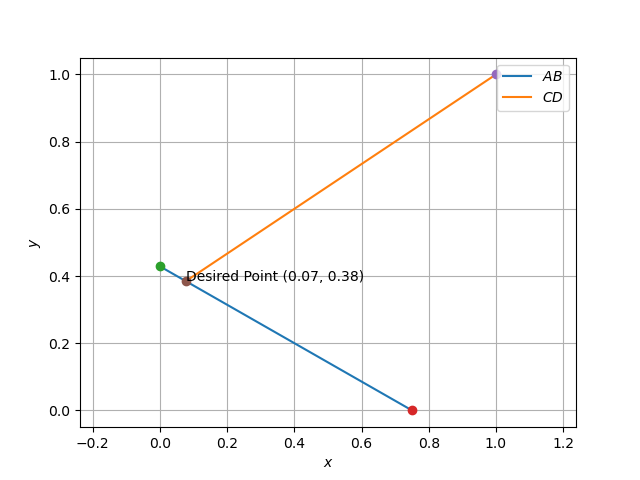
\includegraphics[width=\columnwidth]{Assignment_1}
  \caption{The intercepts of the required line are equal}
\end{figure}
\end{flushleft}
\end{document}
